\documentclass{beamer}
\usepackage{beamerthemesplit}
\usepackage{booktabs}
\RequirePackage{graphicx}
\RequirePackage[italian]{babel}
\usepackage[utf8x]{inputenc}


\title[LOD CB-RS]{Linked Open Data per un Content-based Recommender System}
\institute{ \textbf{Accesso intelligente alle informazioni ed \\ elaborazione del linguaggio naturale\\}
~ \\
\begin{small}
Corso di Laurea in Informatica Magistrale
\end{small}}
\author{\textbf{Luciano Quercia}\\
\textbf{Simone Rutigliano}}
\date{\tiny{\today}}


%\usetheme{Hannover}
\usetheme{Copenhagen}
\usecolortheme{seahorse}
\usecolortheme{rose}
%\usetheme{Frankfurt}
%\usecolortheme{beetle}

%\useoutertheme[subsection=false]{smoothbars}
%\useoutertheme[subsection=false]{smoothtree}
\useoutertheme{shadow}
\setbeamercovered{dynamic}

\pgfdeclareimage[height=1cm]{logo}{figure/logo}
\logo{\pgfuseimage{logo}}


\begin{document}

%%%%%%%%%%%%%%%%%%%%%%%%%%%%%%%%%%%%%%%%%%%%%%%%%%%%%

\begin{frame}
\maketitle
\end{frame}

%%%%%%%%%%%%%%%%%%%%%%%%%%%%%%%%%%%%%%%%%%%%%%%%%%%%%

\begin{frame}
\frametitle{Outline}
\tableofcontents
\end{frame}

%%%%%%%%%%%%%%%%%%%%%%%%%%%%%%%%%%%%%%%%%%%%%%%%%%%%%

\section{Obiettivi}
\begin{frame}
\frametitle{Obiettivi}
\begin{itemize}
\item Realizzazione di un content-based recommender system
\item Basato sulla Linked Open Data Cloud
\item Utilizzando il formalismo RDF
\end{itemize}
\end{frame}

%%%%%%%%%%%%%%%%%%%%%%%%%%%%%%%%%%%%%%%%%%%%%%%%%%%%%

\begin{frame}
\frametitle{Content-based Recommender System}
Il sistema stabilisce a priori la distanza trai film al fine di raccomandare i più simili alle preferenze dell'utente 

\begin{figure}
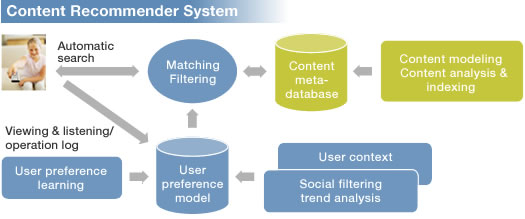
\includegraphics[width=.8\textwidth]{figure/cbrs.jpg}
\end{figure}

\end{frame}

%%%%%%%%%%%%%%%%%%%%%%%%%%%%%%%%%%%%%%%%%%%%%%%%%%%%%

\begin{frame}
\frametitle{Linked Open Data}
Il più grande \emph{Cloud} al mondo di:
\begin{itemize}
\item dataset semantici
\item fortemente interconnessi
\item descritti attraverso RDF
\end{itemize}
\end{frame}

\begin{frame}
\frametitle{Linked Open Data}
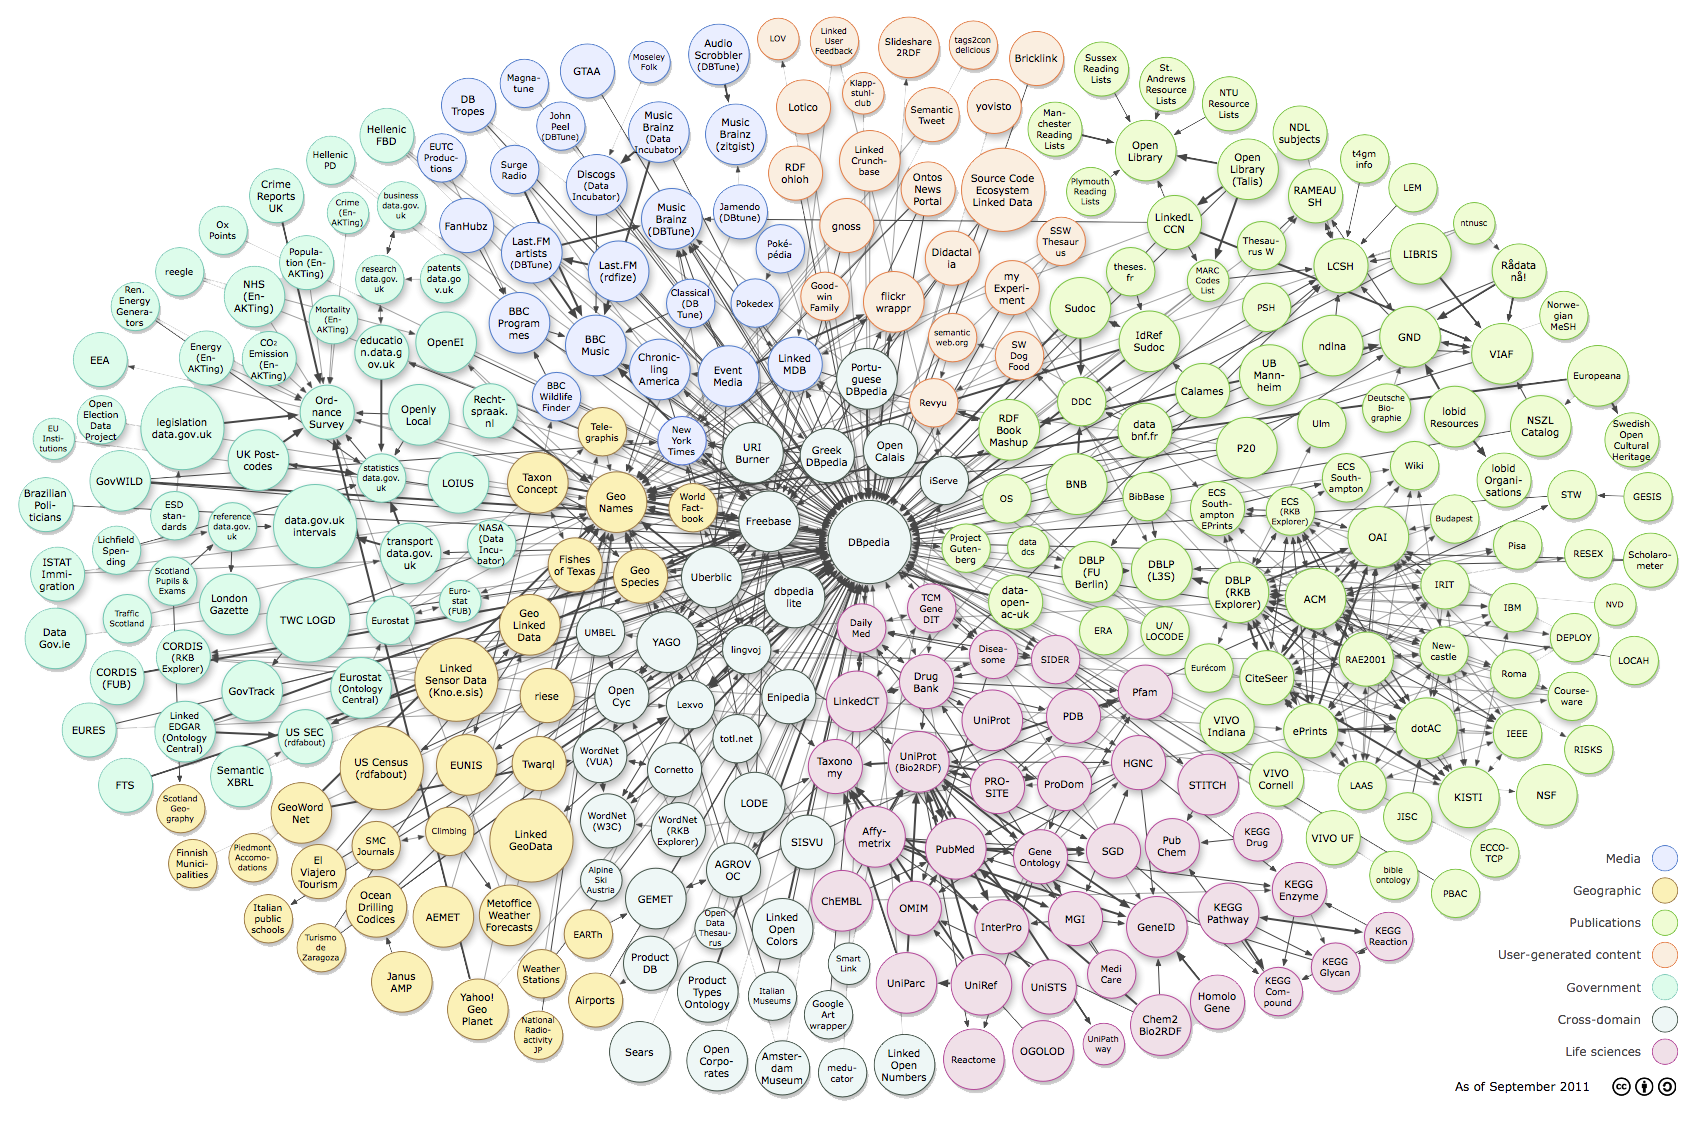
\includegraphics[width=.95\textwidth]{figure/lodcloud}
\end{frame}

%%%%%%%%%%%%%%%%%%%%%%%%%%%%%%%%%%%%%%%%%%%%%%%%%%%%%

\begin{frame}
\frametitle{Resource Description Framework}
Strumento base proposto da \emph{W3C} per la codifica, lo scambio e il riutilizzo di metadati strutturati.

L'RDF Data Model si basa su tre principi chiave:
\begin{enumerate}
\item Qualunque cosa può essere identificata da un (URI)
\item utilizzare il linguaggio meno espressivo per definire qualunque cosa
\item Qualunque cosa può dire qualunque cosa su qualunque cosa
\end{enumerate}
\end{frame}

%%%%%%%%%%%%%%%%%%%%%%%%%%%%%%%%%%%%%%%%%%%%%%%%%%%%%

\section{Progetto}

\subsection{Sorgente dati}

\begin{frame}
\frametitle{DBPedia}
Fulcro della LODC
Trasformazione in RDF di Wikipedia


"Linked Data is about using the Web to connect related data that wasn't previously linked, or using the Web to lower the barriers to linking data currently linked using other methods. More specifically, Wikipedia defines Linked Data as "a term used to describe a recommended best practice for exposing, sharing, and connecting pieces of data, information, and knowledge on the Semantic Web using URIs and RDF."
\begin{figure}

\includegraphics[width=.30\textwidth]{figure/dbpedia_logo}
\end{figure}
\end{frame}

\begin{frame}
\frametitle{Proprietà estratte}
Per la raccomandazione di film, abbiamo estratto le seguenti proprietà
\begin{columns}
\column[t]{5cm}
\begin{itemize}
\item studio
\item music
\item music composer
\item writer
\item editing
\item director
\end{itemize}
\column[t]{5cm}
\begin{itemize}
\item subject
\item starring
\item productor
\item writer
\item cinematography
\end{itemize}
\end{columns}
\end{frame}

%%%%%%%%%%%%%%%%%%%%%%%%%%%%%%%%%%%%%%%%%%%%%%%%%%%%%

\subsection{Realizzazione}

%%%%%%%%%%%%%%%%%%%%%%%%%%%%%%%%%%%%%%%%%%%%%%%%%%%%%

\begin{frame}
\frametitle{Grafo delle Risorse}
Attraverso query SPARQL sono state estratte tutte le triple che avevano proprietà nota e un film come soggetto
È stato generato il grafo relle risorse
\end{frame}

%%%%%%%%%%%%%%%%%%%%%%%%%%%%%%%%%%%%%%%%%%%%%%%%%%%%%

\begin{frame}
\frametitle{Grafo dei Film}
Tutte le risorse non film
\end{frame}

%%%%%%%%%%%%%%%%%%%%%%%%%%%%%%%%%%%%%%%%%%%%%%%%%%%%%

\subsection{Fattori}

%%%%%%%%%%%%%%%%%%%%%%%%%%%%%%%%%%%%%%%%%%%%%%%%%%%%%

\begin{frame}
\frametitle{Distanze}
Sono state applicate 4 distanze su grafo:

\begin{itemize}
\item Direct
\item Combinated
\item Direct Weighted 
\item Combinated Weighted
\end{itemize}
\end{frame}

%%%%%%%%%%%%%%%%%%%%%%%%%%%%%%%%%%%%%%%%%%%%%%%%%%%%%

\begin{frame}
\frametitle{Rappresentazione del profilo}
Il profilo è stato rappresentato in 2 modi:

\begin{itemize}
\item[Simple] Insieme di film positivi per l'utente
\item[Weighted] Ogni film influisce, positivamente o negativamente, alle raccomandazioni, secondo il voto ricevuto
\end{itemize}


\end{frame}

%%%%%%%%%%%%%%%%%%%%%%%%%%%%%%%%%%%%%%%%%%%%%%%%%%%%%

\subsection{Output}

%%%%%%%%%%%%%%%%%%%%%%%%%%%%%%%%%%%%%%%%%%%%%%%%%%%%%

\begin{frame}
\frametitle{Raccomandazioni}
\end{frame}

%%%%%%%%%%%%%%%%%%%%%%%%%%%%%%%%%%%%%%%%%%%%%%%%%%%%%

\section{Sperimentazione}
\subsection{Dataset}

%%%%%%%%%%%%%%%%%%%%%%%%%%%%%%%%%%%%%%%%%%%%%%%%%%%%%

\begin{frame}
\frametitle{MovieLens}
\end{frame}

%%%%%%%%%%%%%%%%%%%%%%%%%%%%%%%%%%%%%%%%%%%%%%%%%%%%%

\subsection{Protocollo Sperimentale}

%%%%%%%%%%%%%%%%%%%%%%%%%%%%%%%%%%%%%%%%%%%%%%%%%%%%%

\begin{frame}
\frametitle{Protocollo Sperimentale}
\end{frame}

%%%%%%%%%%%%%%%%%%%%%%%%%%%%%%%%%%%%%%%%%%%%%%%%%%%%%

\begin{frame}
\frametitle{Metriche}
\end{frame}

%%%%%%%%%%%%%%%%%%%%%%%%%%%%%%%%%%%%%%%%%%%%%%%%%%%%%

\subsection{Risultati}

%%%%%%%%%%%%%%%%%%%%%%%%%%%%%%%%%%%%%%%%%%%%%%%%%%%%%

\begin{frame}
\frametitle{Risultati}
\end{frame}

%%%%%%%%%%%%%%%%%%%%%%%%%%%%%%%%%%%%%%%%%%%%%%%%%%%%%

\section{Conclusioni e sviluppi futuri}
\begin{frame}
\frametitle{Conclusioni e sviluppi futuri}
\end{frame}

%%%%%%%%%%%%%%%%%%%%%%%%%%%%%%%%%%%%%%%%%%%%%%%%%%%%%

\begin{frame}
\frametitle{TEPaC}
TEPaC

\emph{Transductive Emerging Pattern based Classifier}

\begin{itemize}
\item classificatore di strutture logiche
\item basato su pattern emergenti
\item utilizza un approccio trasduttivo
\end{itemize}

\end{frame}

%%%%%%%%%%%%%%%%%%%%%%%%%%%%%%%%%%%%%%%%%%%
%%%%%%%%%%%%%%%%%%%%%%%%%%%%%%%%%%%%%%%%%%%
%%%%%%%%%%%%%%%%%%%%%%%%%%%%%%%%%%%%%%%%%%%

\subsection{Document Image Understanding}
\begin{frame}
\frametitle{Document Image Understanding}

\begin{columns}
\begin{column}{0.6\textwidth}

\begin{itemize}
\item<1-> Comprensione automatizzata di documenti cartacei
\item<2-> La maggior parte della conoscenza mondiale si trova su supporti cartacei
\begin{itemize}
\item Libri
\item Documenti
\item Giornali
\end{itemize}
\item<3-> La digitalizzazione offre innumerevoli vantaggi
\end{itemize}
\end{column}

\begin{column}{0.2\textwidth}
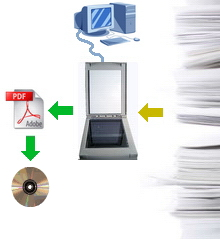
\includegraphics[width=3cm]{figure/diu.jpg}
\end{column}

\end{columns}

\end{frame}


%%%%%%%%%%%%%%%%%%%%%%%%%%%%%%%%%%%%%%%%%%%
%%%%%%%%%%%%%%%%%%%%%%%%%%%%%%%%%%%%%%%%%%%
%%%%%%%%%%%%%%%%%%%%%%%%%%%%%%%%%%%%%%%%%%%


\begin{frame}
\begin{scriptsize}

\begin{columns}
\begin{column}{0.4\textwidth}
	\begin{tabular}{c | ccc}
	\toprule
	 & \multicolumn{3}{c}{$minSup\ (\%)$} \\
	$minGR$ & 30 & 40 & 50 \\
	\hline
	1  & 528032 & 344798 & 254805 \\
	2  & 523274 & 341534 & 252355 \\
	8  & 516958 & 336733 & 248658 \\
	64 & 513503 & 334292 & 246843 \\
	\bottomrule
	\end{tabular}
Dataset TPAMI
	\vspace{8 mm}
	
	\begin{tabular}{c | ccc}
	\toprule
	 & \multicolumn{3}{c}{$minSup\ (\%)$} \\
	$minGR$ & 10 & 20 & 30 \\
	\hline
	1  & 386996 & 176407 & 114492 \\
	2  & 382639 & 173372 & 112476 \\
	8  & 376645 & 169406 & 109814 \\
	64 & 374736 & 167742 & 108595 \\
	\bottomrule
	\end{tabular}
Dataset ICML

\end{column}

\begin{column}{0.4\textwidth}
	\begin{tabular}{c | ccc}
	\toprule
	 & \multicolumn{3}{c}{$minSup\ \ (\%)$} \\
	$minGR$ & 10 & 20 & 30 \\
	\hline
	1  & 128327 & 88684 & 58603 \\
	2  & 126840 & 87644 & 58091 \\
	8  & 122591 & 84208 & 55718 \\
	64 & 121363 & 82980 & 54490 \\
	\bottomrule
	\end{tabular}
Dataset BG

\end{column}
\end{columns}

\end{scriptsize}
\end{frame}


\begin{frame}
\begin{center}
Grazie per l'attenzione.
\end{center}
\end{frame}
\end{document}
